\subsection{Authentication screen}
The authentication screen, containing the forms to login and register in the service, is the one that appears when the user opens for the first time the application (after an initial onboard screen).
In the login section, as shown in the below figure, if a user is using an iOS device, he/she could also login/register with Apple ID, or even continue without registration (possible also for Android OS users).
In the registration screen, there is also the possibility to register with already having a family ID, in this way once the user enters in the application, on the homepage he/she will have could view the products of all family members.\newline

\vspace*{-0.3cm}
\begin{figure}[H]
  \begin{minipage}{0.5\textwidth}
  \centering
    \includegraphics[width=42.mm,scale=0.9]{./Images//Mobile_mocks/Login.png}
    \vspace*{-0.3cm}
    \caption{Mobile Login page}
    \end{minipage}
\hfill
   \begin{minipage}{0.5\textwidth}
     \centering
     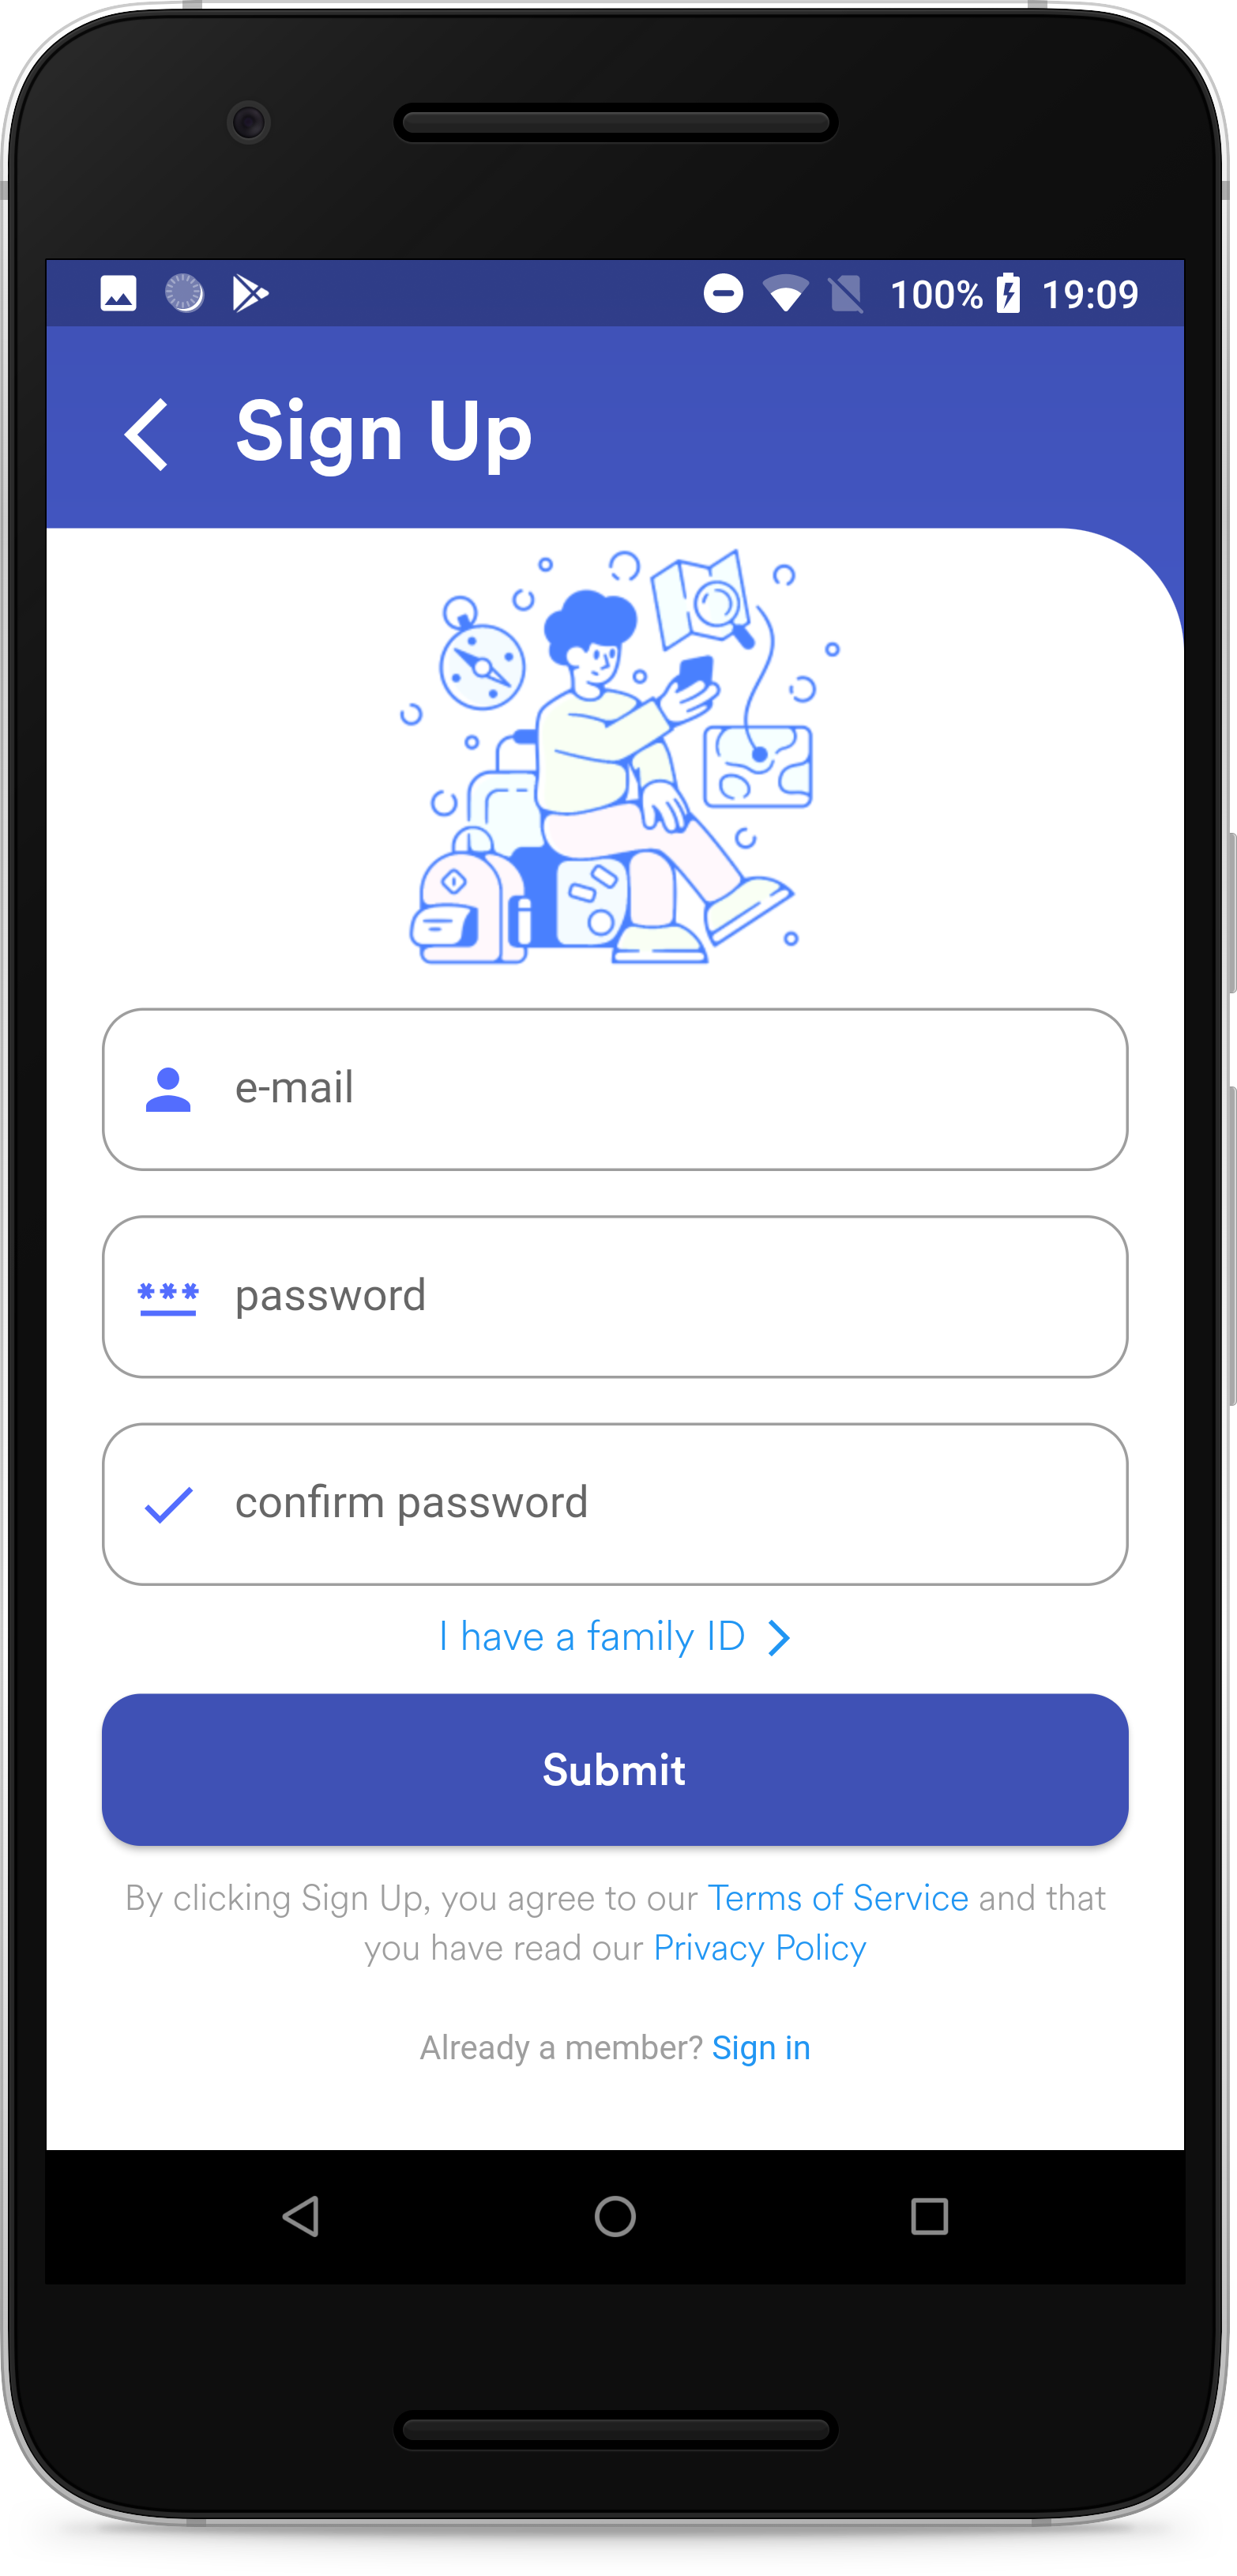
\includegraphics[width=42mm,scale=0.9]{./Images//Mobile_mocks/registration.png}
     \vspace*{-0.3cm}
     \caption{Mobile Registration page}
   \end{minipage}
\end{figure}

\vspace*{-0.3cm}
\begin{figure}[H]
  \centering
    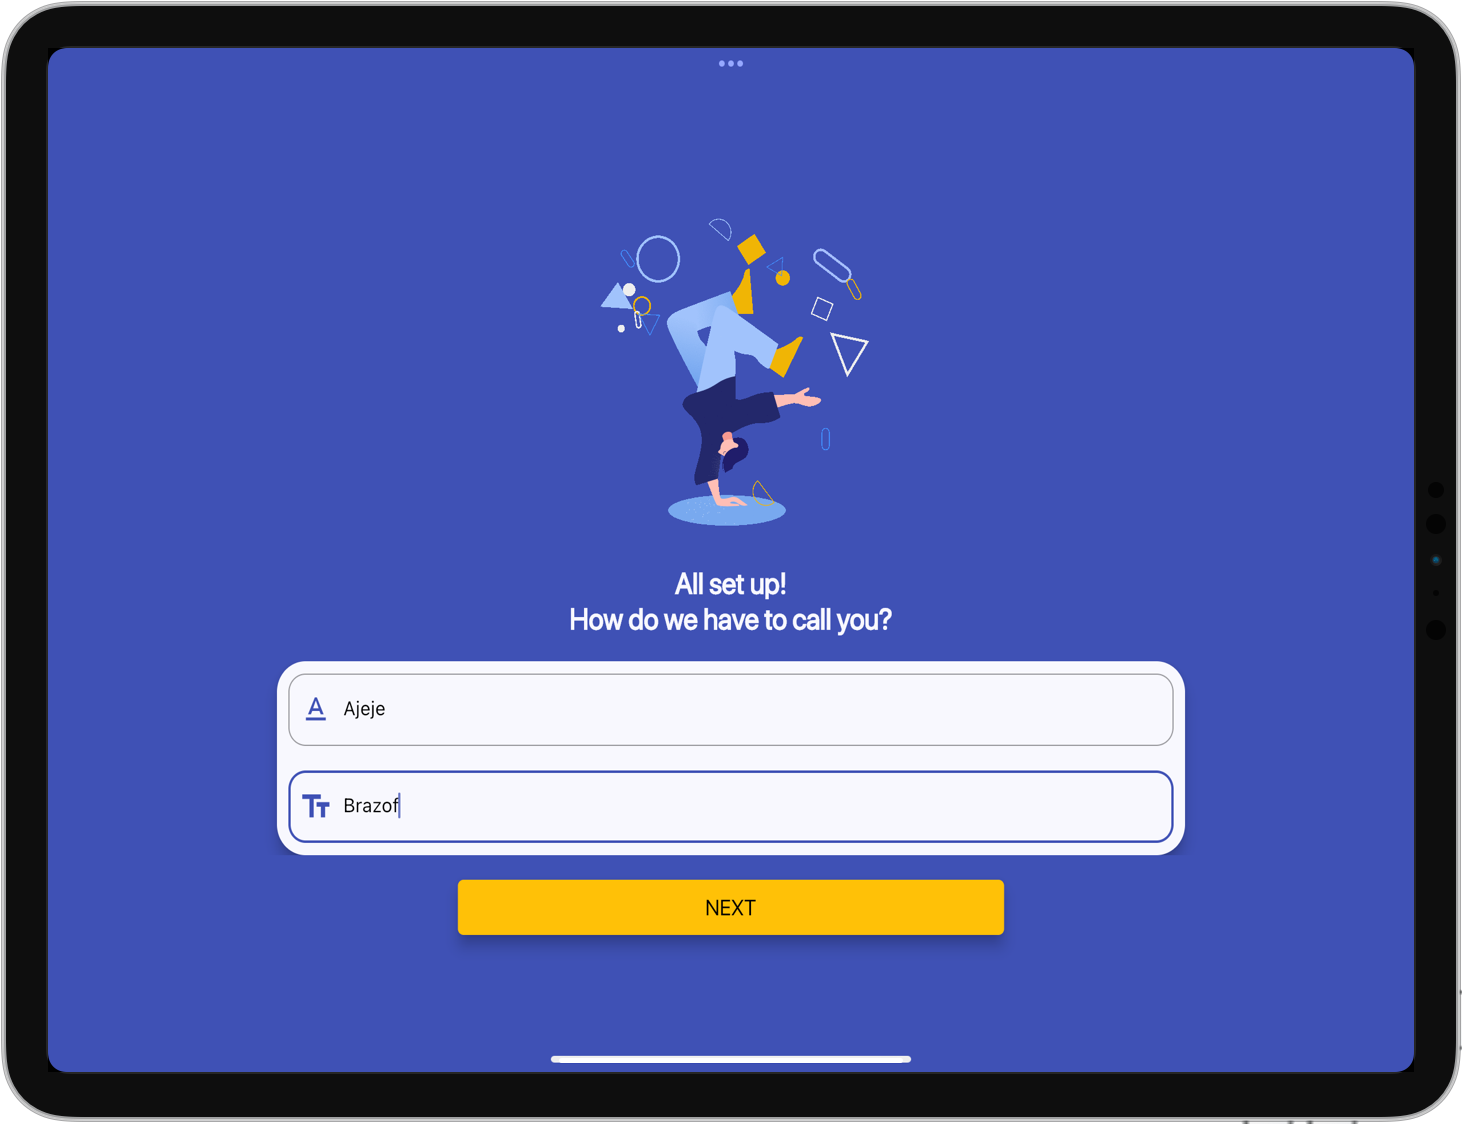
\includegraphics[scale=0.22]{./Images//Tablet_mocks/sign_up3_mod.png}
    \vspace*{-0.3cm}
    \caption{Tablet set display name page}
\end{figure}

